% !TeX encoding = UTF-8

\documentclass{LTHtwocol} % Use this when you work on your report.
% \documentclass[final]{LTHtwocol} % Use this for the final version.
                                   % It will remove page numbers and
                                   % markers for overfull boxes.
                                   % There really shouldn't be any of those anyway.

\usepackage[utf8]{inputenc}        
\usepackage{amsmath,amssymb,graphicx}

\usepackage{xcolor}
\usepackage{hyperref} 
\hypersetup{
	colorlinks,
	linkcolor={red!50!black},
	citecolor={blue!50!black},
	urlcolor={blue!80!black}
}

\usepackage{kantlipsum} % Only for the dummy text. Remove for your own report.

\addbibresource{bibliography.bib}

% Document begins here
\begin{document}
\begin{frontmatter}
\title{Algo Trading} % Title of the project.
                      % Note that all reports are in English,
                      %so that our international students can read them.

\author[måns]{Måns Sandsjö}
\author[august]{August Lindberg Brännström}

\email[måns]{ma8332sa-s@student.lu.se}
\email[august]{august.lindberg.brannstrom@student.lth.se}

\begin{abstract}
The goal of this project is to manage a portfolio of OMX Stockholm 30 stocks using optimization. This is done by collecting price data, cleaning it from outliers, predict future prices and covariance between the stocks and then optimize a portfolio based on this information. By using holding and trading constraints to solve a convex optimization problem, as formulated by Boyd et. al (2007) for each stock during each trading period, the portfolio is re-balanced with the predictions as parameters. How well the predicted returns and covariance are estimated for the model is measured by calculating the Realized Sharpe Ratio (SR) \& Average turnover. Python is used as the main program for data handling and creating predictions. Initial predictions are calculated based of Simple Moving Average (SMA) and Exponential Moving Average (EMA) on simulated stock data provided for the project. For the upcoming future more sophisticated methods are planned involving Learning to identify these parameters. Using simulated data for a period of 20 years with an initial value of the portfolio at 1 MSEK results in an increase to 1,05 MSEK, with a SR of 0,072 when using SMA. With EMA the same result is 0,9 MSEK with a SR at -0,09.

%    The abstract should be a 200--250 word compact description of your project. What was the objective? Which methods did you use? What was the (main) result?
\end{abstract}

\end{frontmatter}

% Stick to the proposed structure below. Add \subsections{} as appropriate.
% This file compiles on the Automatic Control Department system by typing the
% following into the terminal (while in the directory of the file, and with all
% other files belonging to the template untouched):
% > pdflatex template        
% > biber template
% The first line compiles the .tex file. The second line generates the
% bibliography. Once this is done, you may need to run the first line 1-2
% additional times, for the system to get all cross references right in the
% produced pdf output.

\section{Introduction}
The goal of this project is to manage an optimised portfolio of the 30 most traded stocks in Sweden, OMX stockholm 30. This is done by collecting and evaluating data using holding and trading constraints as formulated by Boyd et. al (2017) to solve a convex optimization problem between each trade period\cite{Boyd}. All trading is simulated using real historical data in a so called backtesting environment. 

The project can be divided into three different sub-tasks:
\begin{itemize}
\item Data gathering \& cleaning
\item Build the convex optimization problem solver
\item Implement functions to create predictions on risk \& return
\end{itemize}

 



%Here you introduce the project. What is the background? What project do you aim at solve? References to prior work? If the project makes a positive or negative environmental, or other solitary, impact, describe it here. Are there any ethical considerations? You might want to reference relevant literature, e.g. \cite{openclosed2, Hellerstein2004, Yun2015}. A general \LaTeX\ guide is available at \cite{latexwiki}. 

\subsection{Data gathering \& cleaning}
The data used is the open price on the stock market for each trading day on all the stocks in OMXS30 for the given time period. By cleaning the data from NaN-values \& outliers one can achieve a higher signal to noise ratio. 

\subsection{Convex optimization problem}
%Förklara hur vi löser de konvexa optimeringsproblemet
Convex optimisation is a part within mathematical optimisation with many applications within areas such as finance and statistical analysis as well as automatic control systems, signal processing and more. With a set of constraint one is able to optimise a convex function to identify its maximum/minimum value highly efficient.\cite{Boyd}

%(source: https://web.stanford.edu/~boyd/cvxbook%/bv_cvxbook.pdf)

Convex optimisation is used for evaluating the fraction, hereby referred to as "weights", of each stock to be invested in for each given time period. The function accounts for the future return subtracted by the different cost and risk associated parameters. This is to be maximised and the outcome of the function is what weights should be used to produce the largest predicted risk adjusted outcome.\cite{Boyd}

\subsection{Predictions on risk \& return}
Initially the predictions of future returns can be estimated using simple moving average, referred to as SMA and exponentially weighted moving average, EMA. These are simple methods that works quite poorly as a mean of predicting the future returns, but they provide a basic understanding of the change of return-rate for a given time period. In practise they are rarely used for stock predictions. 

Methods involving more complex ML-methods are planned to be implemented in the future.

The covariance matrix can be calculated with regards to the returns related to the stocks in the portfolio. It can be viewed as a statistical way to explain the relationship between two stocks.\cite{covar} This is used to calculate the risk parameter to solve the risk adjusted return optimization problem.

\section{Modeling}
%August
% datan har vi skapat en filtermodell som sorterar bort över/under 15%
% Hur vi löser optimeringsproblemet
% Hur vi skapar våra predictioner

\subsection{Data gathering \& cleaning}
Companies added to OMXS30 later than project scope are excluded. The cleaning of data is done by filtering outliers based on abnormal return rates set at an increase or decrease of 15\%. If one stock price change is above this threshold then that entire trading day with all stocks pricing will be excluded.

%Here you present the modeling approach and publish your model. If your model has 63434 parameters, you may not wish to print it in detail. The idea is, however, that another group with your background should be able to reproduce your work -- this goes not only for the modeling aspect.
\subsection{Convex optimization problem}
The function to optimize for is as follows:

\begin{equation}
\begin{split}
&\text{Maximize:}\\
&\hat{r_i }^T w_{i,t+1} - \hat{\phi_i}^{trade}(w_{i,t+1}-w_{i,t})-\hat{\phi_i}^{hold}(w_{i,t+1})\\
&-\gamma \psi_i(w_{i,t+1}) \\
&\text{Subject to:} \\
&1^{T}z_{i,t} = 0\\
&w_{i,t}+z_{i,t} \geq 0
\end{split}
\end{equation}

%snygga till typofgrafin
%Obs: korrigera constraints

These terms are individual for each stock "i" and differ at different times "t".

See parameter description below:

\begin{center}
 \begin{tabular}{||c c||} 
 \hline
 Quantity & Description \\ [0.5ex] 
 \hline\hline
 $\hat{r}$ & Estimated return \\ 
 \hline
 $w$ & Fraction of total portfolio value, weights \\
 \hline
 $z$ & Change of portfolio value \\
 \hline
 $\hat{\phi}$ & Trading- \& Holding- cost term\\
 \hline
 $\gamma$ & Risk aversion parameter  \\
 \hline
 $\psi$ & Estimated risk  \\ [1ex] 
 \hline
\end{tabular}
\end{center}

%Byt från den här fula tabellen till något mer neat.

If one let ${P_{i,t}}$ be the price of stock i at time t then the individual return for a stock i is calculated as:
$$
R_{i,t} = \frac{P_{i,t+1}-P_{i,t}}{P_{i,t}}, \quad \forall i=1,\ldots,n \text{ and } \forall t = 1,\ldots,T.
$$

$P_{i,t+1}$ is unknown so in order to succeed in the portfolio re-balancing predicting this value is essential.

The weight factor $w_{i,t}$ in asset i, at time t is defined as:
$$
w_{i,t} = \frac{h_{i,t}}{v_{t}}, \quad \forall i=1,\ldots,n \text{ and } \forall t = 1,\ldots,T+1.
$$
Where $h_{i,t}$ is the value invested in stock i at time t and $v_{t}$ is the total value of portfolio at time t.

The trading cost $\phi^{trade}$ is assumed to be zero. Holding cost $\phi^{hold}$ is set to zero since shorting assets is deemed out of scope for this project in it's current phase.

Risk aversion parameter $\gamma$ is a fixed value used to scale the importance of the estimated return \& estimated risk.

The parameter $\psi$ is the estimated risk, dependant on the co-variance of the different stocks. 

$z_{i,t}$ denotes the unitless increase or decrease of asset i between time $t$ and $t+1$.  

$$
z_{i,t} = \frac{u_{i,t}}{v_{t}}, \quad \forall i=1,\ldots,n \text{ and } \forall t = 1,\ldots,T.
$$

Where $u_{i,t}$ is the increase or decrease in SEK of asset i between time $t$ and $t+1$ and $v_{t}$ is the portfolio value in SEK.

With the adjustments with regards to trading \& holding cost the function is as follows:

\begin{equation}
 \begin{split}
 &\text{Maximize:}\\
 &\hat{r_i }^T w_{i,t+1}  -\gamma\psi_i(w_{i,t+1}) \\
&\text{Subject \: to:} \\
&1^{T}z_{i,t} = 0\\
&w_{i,t}+z_{i,t} \geq 0
\end{split}
\end{equation}
The first constraint, $1^{T}z_{i,t} = 0$, means that the portfolio stays fully invested. The second constraint, $w_{i,t}+z_{i,t} \geq 0$, limits the portfolio to exclude any shortage of sales, i.e. the portfolio cannot gain value from a declining return. \cite{Boyd}


\subsection{Predictions on risk \& return}
Simple moving average is described in \ref{eq:sma} Where $A^n_t$ = the return of the stock n at period $t$ and $T =$ number of periods.
\begin{equation} 
\label{eq:sma}
 \hat{R}_{t \mid t}^{\mathrm{SMA}} = \frac{A^n_1+A^n_2+...+A^n_t}{T_{SMA}}
\end{equation}
Exponential moving average is shown in equation \ref{eq:ema}. Let $\alpha_{\text{EMA}}\in (0,1)$ and $\tau_{\text{EMA}}$ be the temporal center of mass of the exponential moving average. EMA requires a short period of adjustment. Therefore, for the first two periods it is just regarded as the previous $\hat{R}$ value. \cite{ref:ema}
%beskriv r_hat
\begin{equation}
    \label{eq:ema}
    \hat{R}_{t \mid t}^{\mathrm{EMA}}=\left\{\begin{array}{ll}
    R_{t-1}, & \text { if } t=2 \\
    \alpha_{\mathrm{EMA}} \hat{R}_{t-1 \mid t-1}^{\mathrm{EMA}}+\left(1-\alpha_{\mathrm{EMA}}\right) R_{t-1}, & \text { if } 2<t \leq T\\
    \end{array}\right. 
\end{equation}
\begin{equation}
     \alpha_{\text{EMA}} = 1 - \frac{1}{\tau_{\text{EMA}} + 1}
\end{equation}



\subsection{Model quality}
Model quality is measured primarily by calculating the portfolio's risk adjusted return and it's average turnover. The risk adjusted return is a commonly used metric in finance and is called the Sharpe Ratio,\cite{ref:sharpe} this can be calculated as:

$$
SR = \frac{\overline{R^{P}_{t}}}{\widehat{\sigma}^{P}}.
$$
Where $\overline{R^{P}_{t}}$ is the average realized portfolio return: 

$$
\overline{R^{P}_{t}} = \frac{1}{T}\sum_{t=1}^{T}R_{t}^{P}.
$$
and $\widehat{\sigma}^{P}$ is the realized portfolio volatility:
$$
\widehat{\sigma}^{P} = \sqrt{\frac{1}{T}\sum_{t=1}^{T}(R_{t}^{P}-\overline{R^{P}_{t}})^{2}}.
$$
Average turnover is a measure used to determine how much change is happening within the portfolio, how many transaction that are being made in the portfolio. This value can to some extent represent how much losses the portfolio will have in transaction costs, even if the portfolio re-balancing is not optimizing with trading cost as a parameter. Ideally this value is kept low.

$$
\overline{\text{turnover}} = \frac{1}{T}\sum_{t=1}^{T}\frac{\left\lVert z_{t} \right\rVert_{1} }{2}.
$$
$z_{t}$ is a unitless value of the normalized trades at time t.

%Equations are parts of the text. If they end a sentence, they should end with a dot. If they end a clause, they should end with a comma. You refer to an equation this like: see \eqref{eq:formula}. Note that all units are written in roman type: $\omega=2\pi$~rad/s, $g = 9.81$~m/s$^2$. See \cite{mathslatexwiki} for a tutorial on typesetting maths.

\section{System Design}

% Översikt av hela systemet uttryckt i illustration.

%Describe the control or learning system you have designed.
%Did you build anything? If so, what did you build, and using what production methods. If you built the hardware or were handed it, \emph{a photograph of your gadget is mandatory}. Make sure any figures are referenced from from the text---like this, see Figure~\ref{fig:gadget}---and that they all have a descriptive caption.
%Måns
Python is the main language for developing the code in this project. For data gathering, the financial market platform \textit{Investing.com}, which provides historical data on stock prices, is used. For data handling, the data science library \textit{Pandas} is used. 
\subsection{Overview of the system}
The overview of the system design can be seen in figure \ref{fig:overview}. First, the data is fetched and then sent to the prediction model. Second, the prediction model sends the predicted values to the optimization solver. The solver finds  the best weight distribution of the stocks and the results are lastly calculated.

\begin{figure}[h]
	\centering
	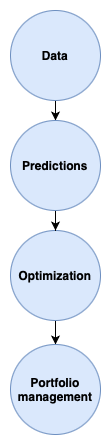
\includegraphics[width=0.2\columnwidth]{Pics/Overview_tree.png}
	\caption{Overview of the project components}
	\label{fig:overview} % Should be placed after the caption!
\end{figure}

\begin{figure}[h]
	\centering
	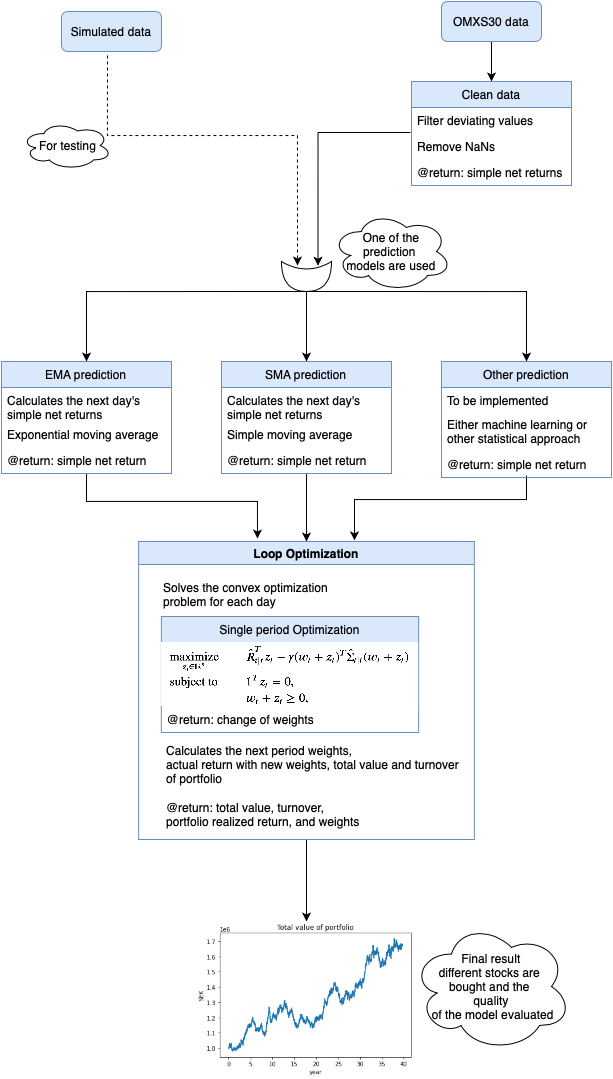
\includegraphics[width=0.7\columnwidth]{Pics/Mod_overview_atm.png}
	\caption{Tree layout of the methods}
	\label{fig:tree_atm} % Should be placed after the caption!
\end{figure}

A detailed layout of the system can be seen in figure \ref{fig:tree_atm}. With the four steps in figure \ref{fig:overview} in mind, the data collection section is either fetched from simulated or real data. Naturally, the real data is cleaned as described above. Next, the prediction part of the expected returns can be split up into simple moving average (SMA), exponential moving average (EMA) or \textit{other prediction model}. To be clear, \textit{other prediction model} is yet to be implemented. Furthermore, the calculated expected returns are sent to the optimization loop where the allocation of the stocks, i.e. weights, are calculated for each day. Finally, the data is evaluated with the model quality parameters and the results are printed and plotted.

%Träd för programmeringen hur alla klasser hänger ihop med varandra
%Data collection – optimering – predictions hur de hänger ihop i ett träd

\section{Implementation}
%skicka in kodsnippar eller pseudokod

\subsection{Data gathering \& cleaning}
The framework is implemented in Python by using data accessible from InvestPy. With Investpy one is given access to Investing.com and their historical stock prices at OMXS30. See details in \ref{fig:DATA_pseud}

\begin{figure}[h]
	\centering
	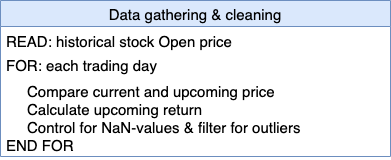
\includegraphics[width=0.7\columnwidth]{Pics/DATA_pseud.png}
	\caption{Pseudocode of Data gathering \& cleaning}
	\label{fig:DATA_pseud} 
\end{figure}

\subsection{Convex optimization solver}
A pseudocode of the convex optimization solver can be seen in figure \ref{fig:optimization}. The code is split up into two methods. First, the optimization method, which calculates the expected net return for each stock and the risk of the post trade portfolio. By subtracting these values, the convex optimization problem then finds the maximum risk adjusted return for the portfolio by using the library CVXPY and its function \textit{Maximize}. The second method, \textit{Loop Optimization}, loops the solver over each day. With the results the method calculates the total value of the portfolio, the portfolio's realized return, and the turnover.

\begin{figure}[h]
	\centering
	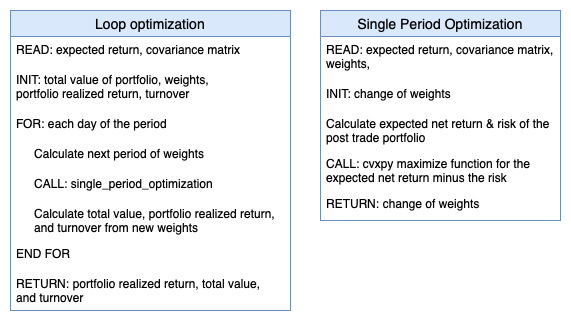
\includegraphics[width=1\columnwidth]{Pics/optimizationPseud.png}
	\caption{Pseudocode of the optimization. Left method is the looping function and right the convex optimization solver.}
	\label{fig:optimization} % Should be placed after the caption!
\end{figure}
\subsection{Predictions}
%Måns skriv om predictions 
At the moment, expected returns are predicted with either SMA or EMA see equation \ref{eq:sma} and \ref{eq:ema}. An pseudocode implementation of SMA and EMA can be seen in figure \ref{fig:SMAnEMApseud}.

\newpage
\begin{figure}[h]
	\centering
	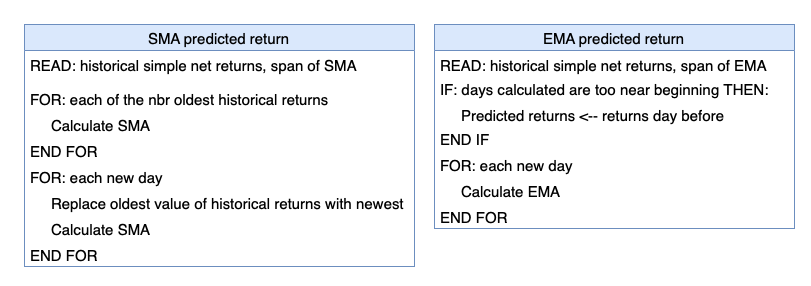
\includegraphics[width=1\columnwidth]{Pics/SMAnEMApseud.png}
	\caption{Pseudocode of the SMA and EMA calculations}
	\label{fig:SMAnEMApseud} % Should be placed after the caption!
\end{figure}


\section{Results}
Looking at the results from the portfolio management, a model to compare the predictions to is the optimization when using only true values. The total value of the portfolio then increases from 1 MSEK to 1.20 MSEK over a 20 year period. See figure \ref{fig:GraphtotValues_TrueValues}. Corresponding model quality values can be seen in the table named \textit{True Values} below. Note that both the average turnover and Sharpe ratio are  annualized.

\begin{center}
 \begin{tabular}{||l l||} 
 \hline
 \textbf{True Values} & \\ [0.5ex] 
 \hline
 Performance Metric & Value\\ [0.5ex] 
 \hline\hline
 Total Value & $=1200850$ SEK \\ 
 \hline
 Average Turnover& $=0.533$ \\
 \hline
 Realized Sharpe Ratio & $=0.261$ \\  [1ex] 
 \hline
\end{tabular}
\end{center}
\begin{figure}[h]
	\centering
	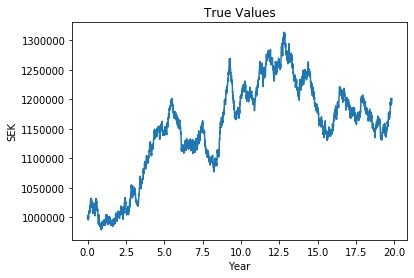
\includegraphics[width=0.8\columnwidth]{Pics/GraphtotValues_TrueValues.jpg}
	\caption{Total value of portfolio, using true values, over 20 years of simulated stock data.}
	\label{fig:GraphtotValues_TrueValues} 
\end{figure}

Using SMA predicted return, the total value of the portfolio increased from 1 MSEK to 1.05 MSEK over a 20 year period. See figure \ref{fig:GraphtotValues_SMA}. The performance metrics is seen in the table named \textit{SMA Predicted Return}.

\begin{center}
 \begin{tabular}{||l l||} 
 \hline
 \textbf{SMA Predicted Return} & \\ [0.5ex] 
 \hline
 Performance Metric & Value\\ [0.5ex] 
 \hline\hline
 Total Value & $=1050350$ SEK \\ 
 \hline
 Average Turnover& $=217.3886$ \\
 \hline
 Realized Sharpe Ratio & $=0.072$ \\  [1ex] 
 \hline
\end{tabular}
\end{center}
\begin{figure}[h]
	\centering
	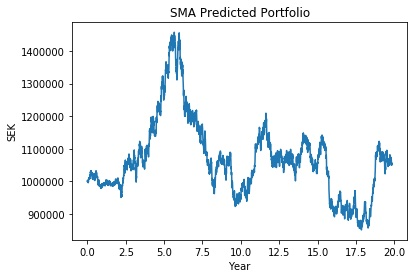
\includegraphics[width=0.8\columnwidth]{Pics/GraphtotValues_SMA.jpg}
	\caption{Total value of portfolio, using SMA predicted returns, over 20 years of simulated stock data.}
	\label{fig:GraphtotValues_SMA} 
\end{figure}

Finally, the EMA predicted return results' can be seen in table named \textit{EMA Predicted Return}. The total value of this portfolio decreased to 0.90 MSEK from 1 MSEK, see figure \ref{fig:GraphtotValues_EMA}.

\begin{center}
 \begin{tabular}{||l l||} 
 \hline
 \textbf{EMA Predicted Return} & \\ [0.5ex] 
 \hline
 Performance Metric & Value\\ [0.5ex] 
 \hline\hline
 Total Value & $=897420$ SEK \\ 
 \hline
 Average Turnover& $=0.7260$ \\
 \hline
 Realized Sharpe Ratio & $=-0.091$ \\  [1ex] 
 \hline
\end{tabular}
\end{center}
\begin{figure}[h]
	\centering
	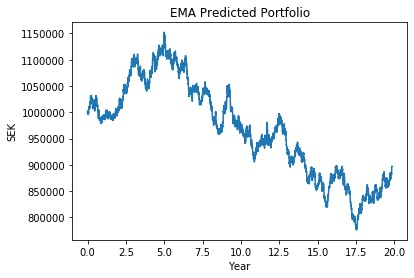
\includegraphics[width=0.8\columnwidth]{Pics/GraphtotValues_EMA.jpg}
	\caption{Total value of portfolio, using EMA predicted return, over 20 years of simulated stock data.}
	\label{fig:GraphtotValues_EMA} 
\end{figure}



\section{Discussion}
\subsection{Initial challenges}
Before the group felt comfortable working with the framework set up by Boyd et. al (2007) further reading within fundamentals of finance and knowledge in stock trading was needed. Working with convex optimization for optimizing the portfolio also required some further studies of the subject. 

Initially Yfinance was planned to be used as the data gathering API for gathering information related to stock price, but due to unstable results and frequent crashes of the program, caused by the API, the group decided to go with Investpy instead.

Examining the results, the prediction models need some development. Especially the SMA prediction with an average turnover of $2170$\% would result in brokerage fees much higher than the anticipated returns.

Similarly, the EMA-portfolio results in a loss with $11.4$\% and a negative Sharpe ratio. To conclude, a new return prediction model is needed for the portfolio management to be successful.

\subsection{Future work}
Previously the group has worked primarily with predictions based on the simulated data, for future work the real stock data from OMXS30 will instead be used. For applying the model to real data the covariance matrix needs to be calculated for each point in time t. Once this is done SMA and EMA can be used for the OMXS30 data, see figure \ref{fig:tree_future}. The result of this will be analysed and after that other more sophisticated means of generating the predictions will be done. 

% Problem vi stött på: Yfinance, 
%samma resultat för predictions även om SMA/EMA använts.

% Diskutera kring de metrics som vi har (sharpe ratio & average turnover)


% Framtida arbete
% Utgick från simulerad data, fortsätter med faktisk data
\clearpage
\begin{figure}[t]
\centering
	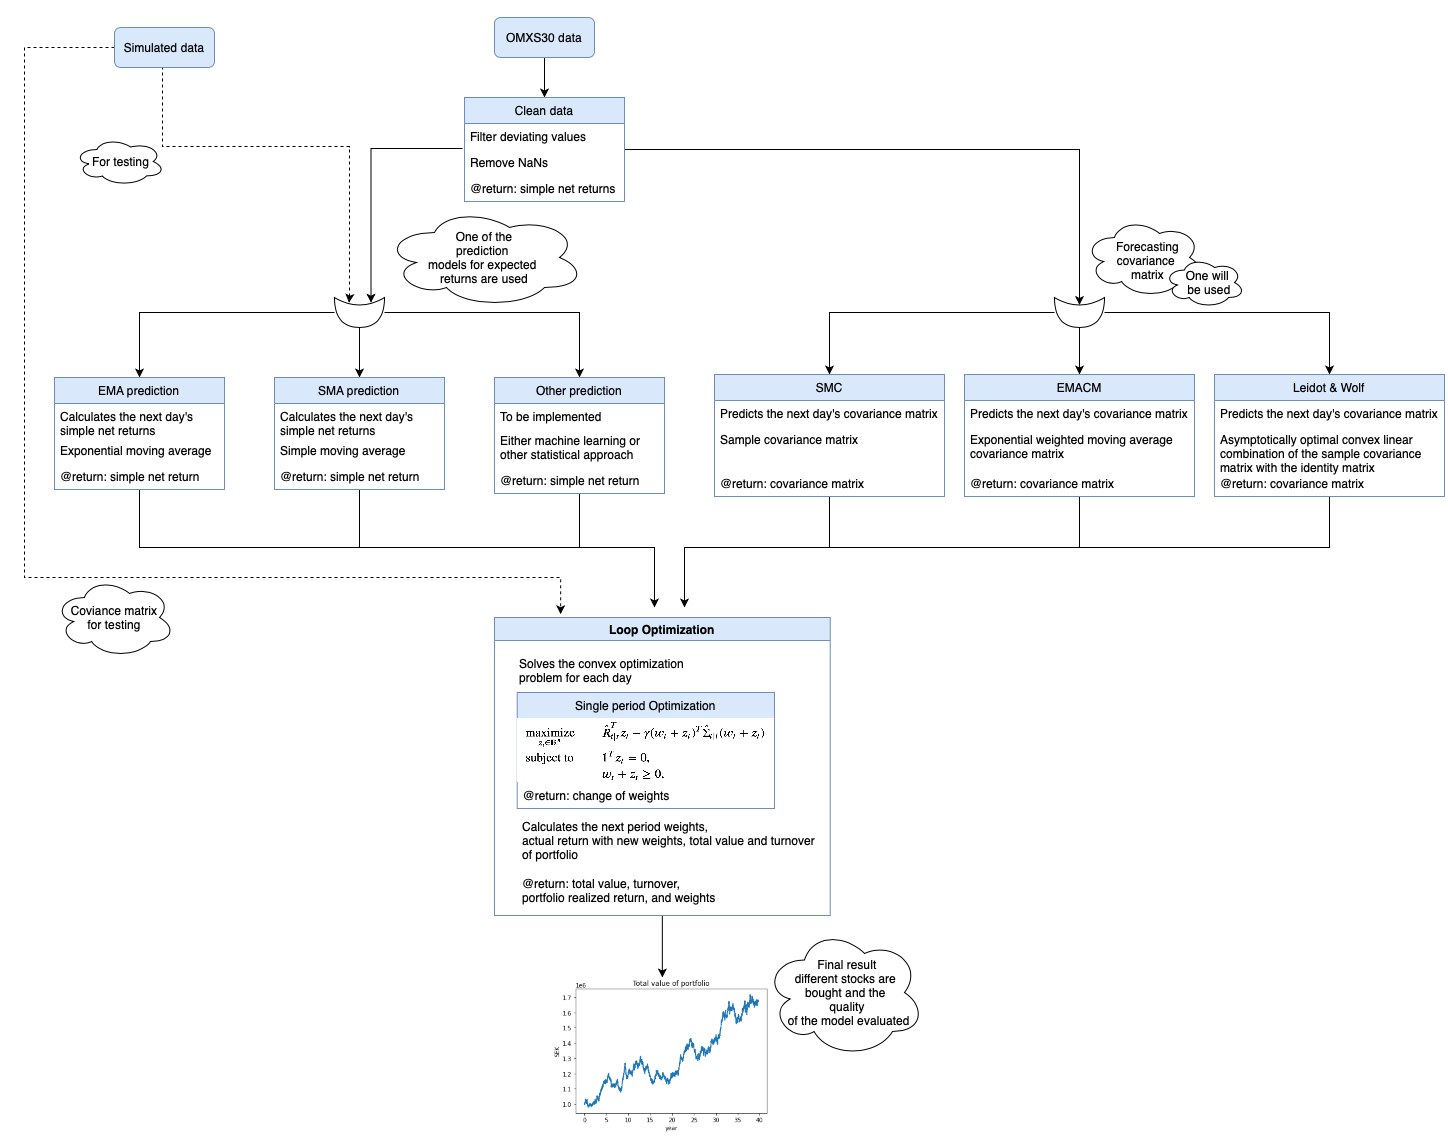
\includegraphics[width=1\textwidth]{Pics/Mod_overview_future.png}
	\begin{centering}
	\caption{Tree overview of the project methods. Right hand side of the figure shows the future work including other prediction for expected returns. The covariance matrix needs to be estimated and the real data will be used}
	\end{centering}
	\label{fig:tree_future} % Should be placed after the caption!
\end{figure}


% Prints cited references
\printbibliography


\end{document}


